\documentclass{report}
\usepackage[T1]{fontenc}
\usepackage[utf8]{inputenc}
\usepackage[english]{babel}
\usepackage{graphicx}
\usepackage{fancyhdr}
\pagestyle{fancy}
\lhead{\textbf{System and device programming}}
\rhead{Laboratory 6}
\lfoot{Enrico Franco}
\rfoot{Politecnico di Torino}
\author{Enrico Franco}
\title{System and Device Programming \\
	Laboratory 6 - Exercise 1}
\begin{document}
\section*{Exercise 1}
In order to install modules and drivers, first it is needed to login as root, for example using command \texttt{sudo -s} on my machine\footnote{Xubuntu 18.04}.

After moving into directory \texttt{hello-5}, with command \texttt{make} it is possible to compile \texttt{hello.c} file as shown in figure~\ref{img:make}.

\begin{figure}[hbtp]
\centering
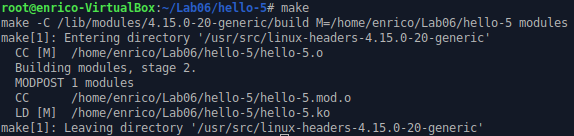
\includegraphics[scale=0.45]{images/es01/make.png}
\caption{make}
\label{img:make}
\end{figure}

Exploiting command \texttt{ls} it is possible to verify if the compilation process has correctly created necessary files and individuate the \texttt{.ko} file (\texttt{hello-5.ko} in this case) which is the one to install as a kernel module. Performing \texttt{lsmod} it is possible to ensure that the module has not been installed yet, and with \texttt{insmod}, which takes the kernel object as an argument, the module should be installed. In order to verify if the module has been installed properly, it is possible to execute command \texttt{lsmod} again.

\begin{figure}[hbtp]
\centering
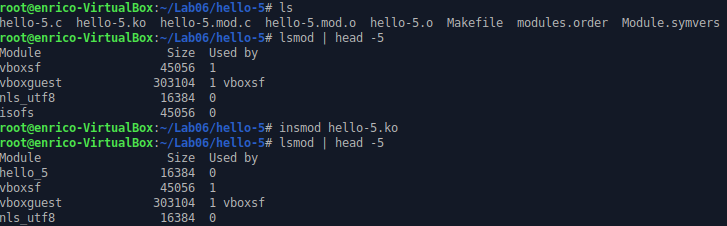
\includegraphics[scale=0.45]{images/es01/insmod_lsmod.png}
\caption{insmod and lsmod}
\label{img:insmod_lsmod}
\end{figure}

The list of possible parameters can be found executing command \texttt{modinfo hello-5.ko} as shown in figure~\ref{img:modinfo}. If the module is installed without any parameter, default ones will be used. Once, the list of parameters has been read, it is possible to install the module inferring some parameters, simply with some assignment statements, as shown on figure~\ref{img:insmod_parameters}.

\begin{figure}[hbtp]
\centering
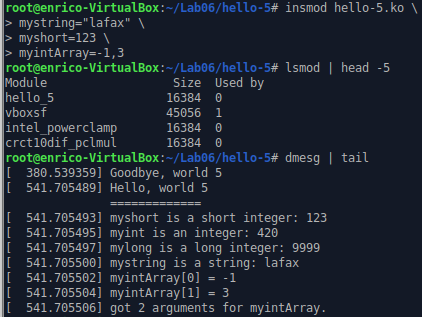
\includegraphics[scale=0.45]{images/es01/insmod_parameters.png}
\caption{insmod with parameters}
\label{img:insmod_parameters}
\end{figure}

\newpage
Parameters are stored in files on \texttt{/sys/module/hello\_5/paramters}, which can be read using command \texttt{cat} for example, as shown in figure~\ref{img:cat_parameters}.

\begin{figure}[hbtp]
\centering
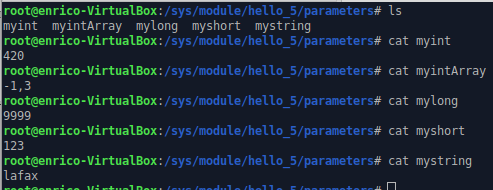
\includegraphics[scale=0.4]{images/es01/cat_parameters.png}
\caption{Parameter values}
\label{img:cat_parameters}
\end{figure}

Using command \texttt{dmesg}, it is possible to view the latest messages generated by modules. Since module \texttt{hello-5} executes some \texttt{printk} concerning parameters on initialization, with \texttt{dmesg} it is possible to see the parameters and their values. \texttt{dmesg} permits to know if the module has been correctly removed, since module \texttt{hello-5} performs a \texttt{printk} in its exiting method, i.e.\@ the one called during module removal.

\begin{figure}[hbtp]
\centering
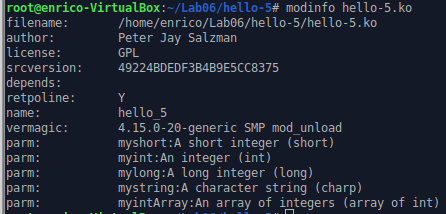
\includegraphics[scale=0.4]{images/es01/modinfo.png}
\caption{modinfo}
\label{img:modinfo}
\end{figure}

\end{document}